\documentclass[12pt]{article}%
\usepackage{amsmath}
\usepackage{graphicx}


\begin{document}

\newcommand\scalemath[2]{\scalebox{#1}{\mbox{\ensuremath{\displaystyle #2}}}}
\title{Machine Learning \protect\\ Assignment 2 \protect\\ CLO2} 
\author{Ida Bagus Dwi Satria Kusuma \protect\\ 1301140297}
\date{\today}
\maketitle

\begin{enumerate}
	\item \par Given data set 1 $(x_i, y_i)$ shown in Table 1.
	
	\begin{enumerate}
		\item (20 points) Build a univariate linear regression model using data set 1 (except p4).
		\par Untuk membuat regresi linear [2]

		\[f(x) = \omega_1 x + \omega_0 \ ,\]

		\par kita perlu mengetahui nilai $\omega_1$ dan $\omega_0$ terlebih dahulu. Untuk mencari nilai $\omega_1$ dan $\omega_0$, kita dapat menggunakan \textit{normal equation} [2]

			\[\begin{pmatrix} N & \sum_i x_i\\ \sum_i x_i & \sum_i x_i^2 \end{pmatrix} \begin{pmatrix} \omega_0 \\ \omega_1 \end{pmatrix} = \begin{pmatrix} \sum_i y_i\\ \sum_i x_i y_i \end{pmatrix}\]

		\par yang kemudian disesuaikan untuk mencari nilai $\omega_1$ dan $\omega_0$ ,

			\[\begin{pmatrix} \hat{\omega_0} \\ \hat{\omega_1} \end{pmatrix} = \begin{pmatrix} N & \sum_i x_i\\ \sum_i x_i & \sum_i x_i^2 \end{pmatrix}^{-1} \begin{pmatrix} \sum_i y_i\\ \sum_i x_i y_i \end{pmatrix}\]

		\par Setelah melakukan perhitungan, diketahui fakta berikut :

			\[N = 6 \ , \ \sum_i x_i = 33.2 \ , \ \sum_i x_i^2 = 209.74 \ , \ \sum_i y_i = 19.2 \ , \ \sum_i x_i y_i = 102.5\]

		\par Kemudian, dengan menggunakan persamaan \texit{normal equation}[2], kita memperoleh 

			% \begin{equation}
			\begin{align*}
				\begin{pmatrix} \hat{\omega_0} \\ \hat{\omega_1} \end{pmatrix} & = \begin{pmatrix} 6 & 33.2\\ 33.2 & 209.74\end{pmatrix}^{-1} \begin{pmatrix} 19.2\\ 102.5 \end{pmatrix} \\
			\end{align*}
			% \end{equation}

		\par Diketahui :

			% \begin{equation}
			\begin{align*}
				\begin{pmatrix} 6 & 33.2\\ 33.2 & 209.74 \end{pmatrix} ^{-1} & = \frac{1}{1258.44-1102.24} \begin{pmatrix} 209.74 & -33.2\\ -33.2 & 6 \end{pmatrix} \\ \\
				& = \frac{1}{156.2} \begin{pmatrix} 209.74 & -33.2\\ -33.2 & 6 \end{pmatrix} \\ \\
				& = \begin{pmatrix} 1.343 & -0.213\\ -0.213 & 0.038 \end{pmatrix}
			\end{align*}
			% \end{equation}

		\par Maka : 

			\begin{align*}
				\begin{pmatrix} \hat{\omega_0} \\ \hat{\omega_1} \end{pmatrix} & = \begin{pmatrix} 6 & 33.2\\ 33.2 & 209.74\end{pmatrix}^{-1} \begin{pmatrix} 19.2\\ 102.5 \end{pmatrix} \\ \\
				& = \begin{pmatrix} 1.343 & -0.213\\ -0.213 & 0.038 \end{pmatrix} \begin{pmatrix} 19.2\\ 102.5 \end{pmatrix} \\ \\
				& = \begin{pmatrix}3.994 \\ -0.1437 \end{pmatrix}
			\end{align*}

			\begin{align*}
				\hat{\omega_0} & = 3.994 \\ 
				\hat{\omega_1} & = -0.1437
			\end{align*}

		\par Dari perhitungan tersebut, kita telah mendapatkan nilai $\omega_0$ dan $\omega_1$. Maka model regersi linearnya adalah 

			\begin{align*}
				f(x) = -0.1437x + 3.994
			\end{align*} 

		\par Jika digambarkan pada grafik, maka akan seperti ini

		\par 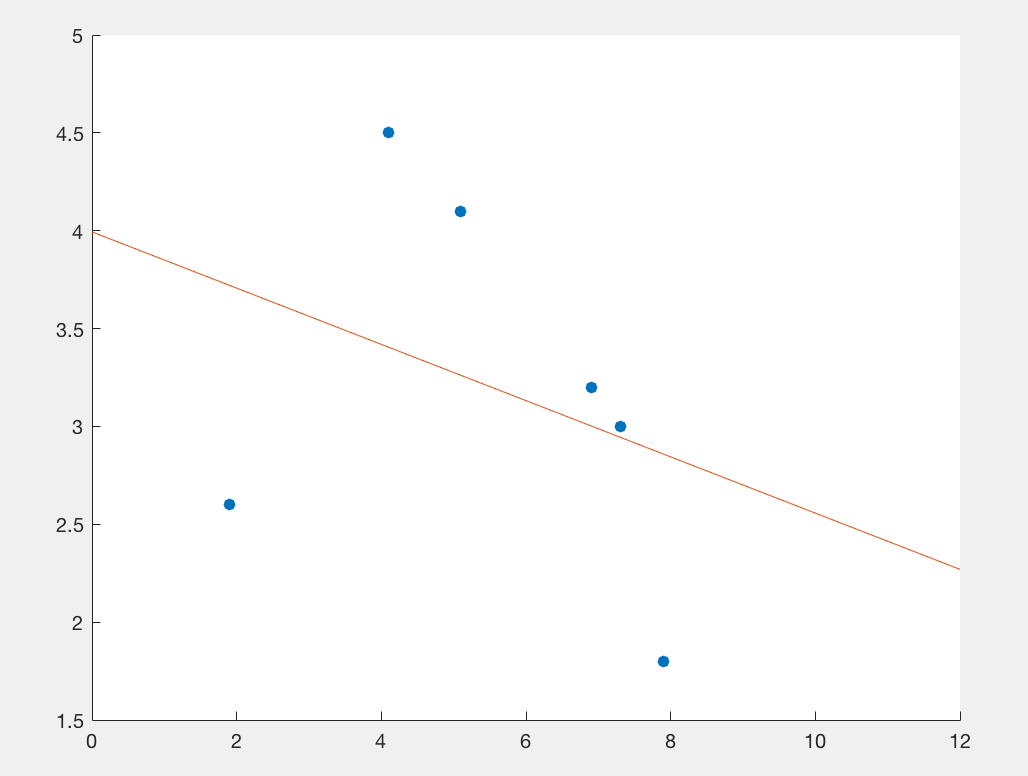
\includegraphics[width=10cm]{ass2clo2fig1} 

		\item (5 points) Predict the $y_4 $that is the $y$ value of p4 using univariate linear regression model in 15(a).

		\par Diketahui nilai x adalah 6.0, maka

			\begin{align*}
				f(x) & = -0.1437(6.0) + 3.994 \\
				& = 3.1318
			\end{align*}

		\par Jadi nilai $y_4$ adalah $3.1318$

		\item (20 points) Build a univariate non-linear regression model using data set 1 (except p4). (Hints: use m degree polynomial. It is up to you in selecting m value.)

		\par Diketahui fungsi polynomial dengan derajat m = 7 adalah 

			\[y = \omega_0 + \omega_1x + \omega_2x^2 + \omega_3x^3 + \omega_4x^4 + \omega_5x^5 + \omega_6x^6 + \omega_7x^7\]


		\par Untuk menghitung masing-masing nilai a, kita dapat menggunakan kembali \textit{normal equation} dengan menyesuaikan matrix inputan, menjadi

		\[
		\scalemath{0.75}{
		\begin{pmatrix} n & \sum x_i & \sum x_i^2 & \sum x_i^3 & \sum x_i^4 & \sum x_i^5 & \sum x_i^6 & \sum x_i^7\\ \sum x_i & \sum x_i^2 & \sum x_i^3 & \sum x_i^4 & \sum x_i^5 & \sum x_i^6 & \sum x_i^7 & \sum x_i^8\\ \sum x_i^3 & \sum x_i^4 & \sum x_i^5 & \sum x_i^6 & \sum x_i^7 & \sum x_i^8 & \sum x_i^9 & \sum x_i^{10} \\ \sum x_i^4 & \sum x_i^5 & \sum x_i^6 & \sum x_i^7 & \sum x_i^8 & \sum x_i^9 & \sum x_i^{10} & \sum x_i^{11} \\ \sum x_i^5 & \sum x_i^6 & \sum x_i^7 & \sum x_i^8 & \sum x_i^9 & \sum x_i^{10} & \sum x_i^{11} & \sum x_i^{12} \\ \sum x_i^6 & \sum x_i^7 & \sum x_i^8 & \sum x_i^9 & \sum x_i^{10} & \sum x_i^{11} & \sum x_i^{12} & \sum x_i^{13} \\ \sum x_i^7 & \sum x_i^8 & \sum x_i^9 & \sum x_i^{10} & \sum x_i^{11} & \sum x_i^{12} & \sum x_i^{13} & \sum x_i^{14} \end{pmatrix} \begin{pmatrix} \omega_0\\ \omega_1\\ \omega_2\\ \omega_3\\ \omega_4\\ \omega_5\\ \omega_6 \\ \omega_7 \end{pmatrix} = \begin{pmatrix} \sum y_i\\ \sum x_i y_i\\ \sum x_i^2 y_i\\ \sum x_i^3 y_i\\ \sum x_i^4 y_i\\ \sum x_i^5 y_i\\ \sum x_i^6 y_i\\ \sum x_i^7 y_i \end{pmatrix} }
		\]

		\[
		\scalemath{0.75}{
		\begin{pmatrix} n & \sum x_i & \sum x_i^2 & \sum x_i^3 & \sum x_i^4 & \sum x_i^5 & \sum x_i^6 & \sum x_i^7\\ \sum x_i & \sum x_i^2 & \sum x_i^3 & \sum x_i^4 & \sum x_i^5 & \sum x_i^6 & \sum x_i^7 & \sum x_i^8\\ \sum x_i^3 & \sum x_i^4 & \sum x_i^5 & \sum x_i^6 & \sum x_i^7 & \sum x_i^8 & \sum x_i^9 & \sum x_i^{10} \\ \sum x_i^4 & \sum x_i^5 & \sum x_i^6 & \sum x_i^7 & \sum x_i^8 & \sum x_i^9 & \sum x_i^{10} & \sum x_i^{11} \\ \sum x_i^5 & \sum x_i^6 & \sum x_i^7 & \sum x_i^8 & \sum x_i^9 & \sum x_i^{10} & \sum x_i^{11} & \sum x_i^{12} \\ \sum x_i^6 & \sum x_i^7 & \sum x_i^8 & \sum x_i^9 & \sum x_i^{10} & \sum x_i^{11} & \sum x_i^{12} & \sum x_i^{13} \\ \sum x_i^7 & \sum x_i^8 & \sum x_i^9 & \sum x_i^{10} & \sum x_i^{11} & \sum x_i^{12} & \sum x_i^{13} & \sum x_i^{14} \end{pmatrix}^{-1} \begin{pmatrix} \sum y_i\\ \sum x_i y_i\\ \sum x_i^2 y_i\\ \sum x_i^3 y_i\\ \sum x_i^4 y_i\\ \sum x_i^5 y_i\\ \sum x_i^6 y_i\\ \sum x_i^7 y_i \end{pmatrix}  = \begin{pmatrix} \omega_0\\ \omega_1\\ \omega_2\\ \omega_3\\ \omega_4\\ \omega_5\\ \omega_6 \\ \omega_7 \end{pmatrix}}
		\]

		\[

		\scalemath{0.7}{
		\begin{gathered}
		\begin{pmatrix} 6 & 33.20 & 209.74 & 1418.996 & 9973.6726 & 71775.16892 & 524733.28 & 3879071.96\\ 33.20 & 209.74 & 1418.996 & 9973.67 & 71775.169 & 524733.28 & 3879071.96 & 28911371.296\\209.7400 & 1418.996 & 9973.67 & 71775.169 & 524733.28 & 3879071.96 & 28911371.296 & 216837140.3 \\ 1418.996 & 9973.67 & 71775.169 & 524733.28 & 3879071.96 & 28911371.3 & 216837140.3 & 1634456718.7 \\ 9973.67 & 71775.169 & 524733.28 & 3879071.96 & 28911371.3 & 216837140.3 & 1634456718.72 & 12371294954.18 \\ 71775.17 & 524733.28 & 3879071.96 & 28911371.3 & 216837140.32 & 1634456718.72 & 12371294954.18 & 93972084048.93 \\ 524733.28 & 3879071.96 & 28911371.3 & 216837140.3 & 1634456718.72 & 12371294954.18 & 93972084048.93 & 716039188528.61 \\ 3879071.96 & 28911371.3 & 216837140.3 & 1634456718.72 & 12371294954.18 & 93972084048.93 & 716039188528.61 & 5471265871016.91 \end{pmatrix}^{-1} \\ \times \begin{pmatrix} 19.20\\ 102.50\\ 616.23\\ 3977.60\\ 26863.17\\ 187052.11\\ 1330540.79\\ 9609566.42 \end{pmatrix}  = \begin{pmatrix} \omega_0\\ \omega_1\\ \omega_2\\ \omega_3\\ \omega_4\\ \omega_5\\ \omega_6 \\ \omega_7 \end{pmatrix}
		\end{gathered}
		}
		\]

		\par Sehingga kita mendapatkan nilai-nilai $\omega$ yaitu 

		\begin{gathered}
			\omega_0 = 54727.64 , \omega_1 = -68068.79 ,\omega_2 = 30076.49 , \\ \omega_3 = -5467.20,\omega_4 = 143.43,\omega_5 = 87.41 , \omega_6 = -11.59,\omega_7 = 0.45
		\end{gathered}

		\par Berikut adalah gambar grafik regresi menggunakan polynomial dengan derajat m = 2 sampai m = 7. Jika diperhatikan baik-baik, semakin tinggi nilai m, semakin akurat garis dengan titik-titik pada grafik.

		\par 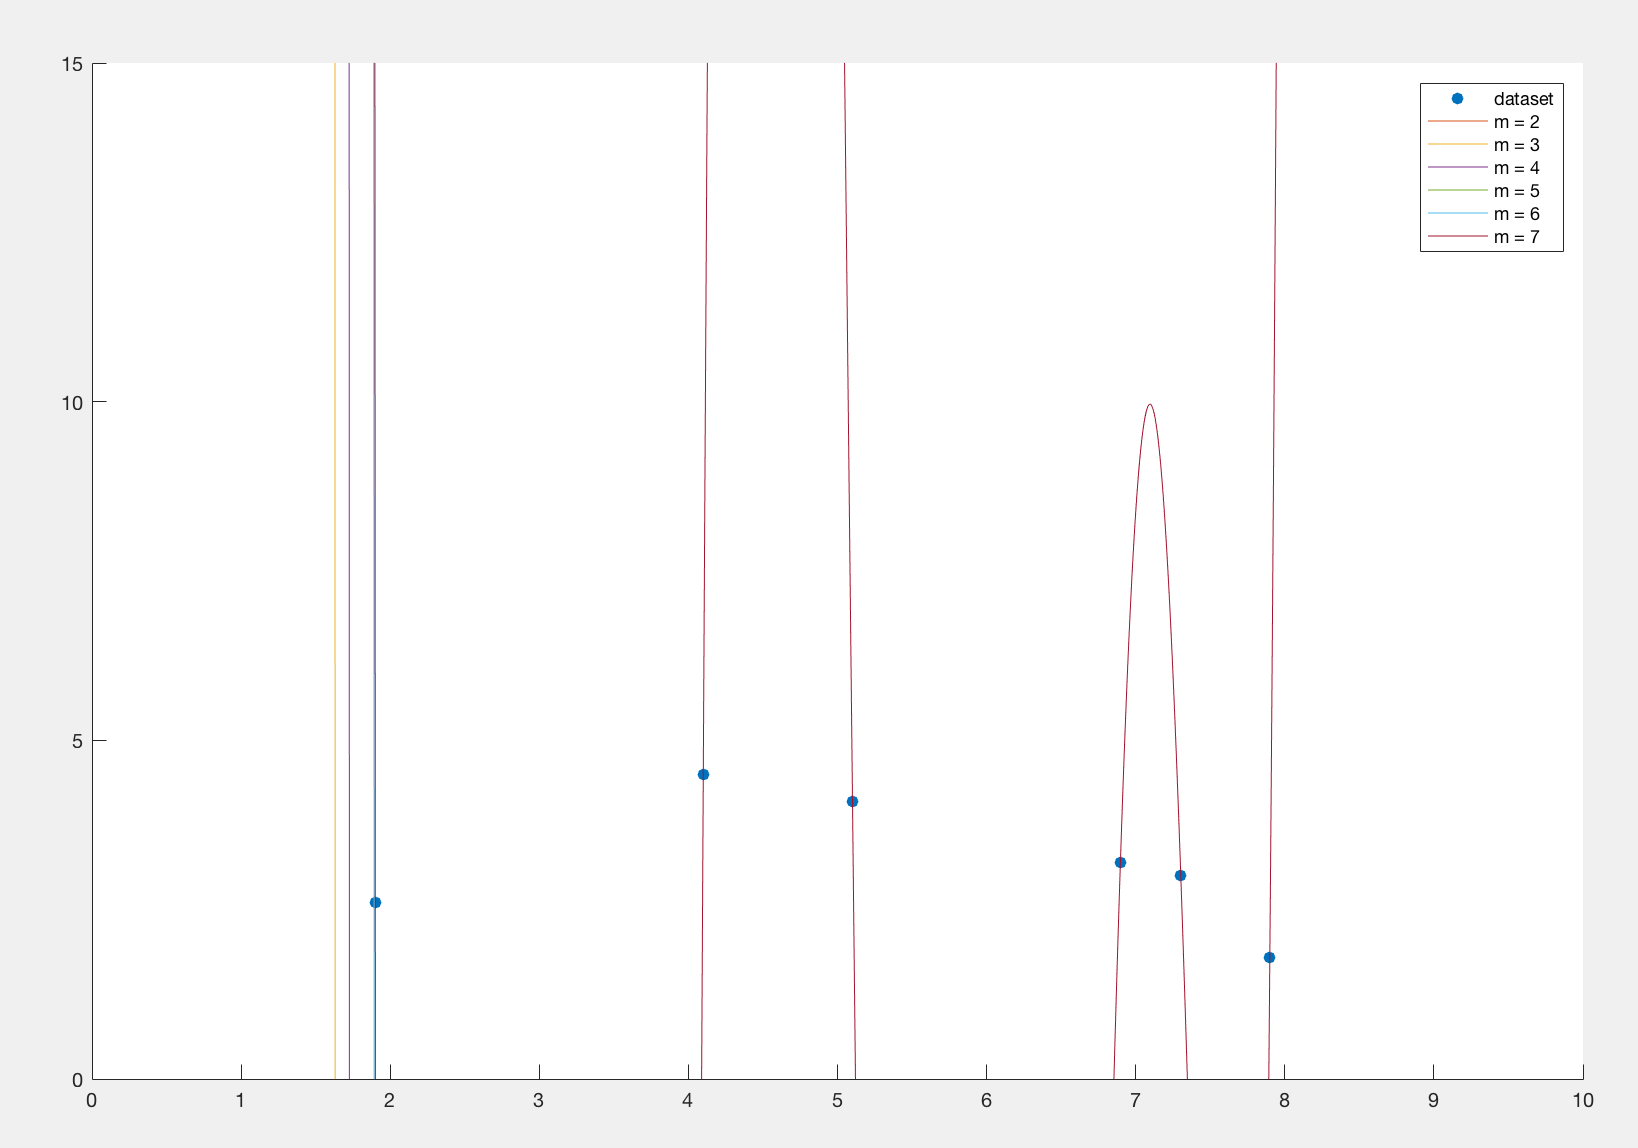
\includegraphics[width=12cm]{ass2clo2fig3} 

		\item (5 points) Predict the y4 that is the y value of p4 using univariate non-linear regression model in 15(c).

		\par Menggunakan persamaan

			\[y = \omega_0 + \omega_1x + \omega_2x^2 + \omega_3x^3 + \omega_4x^4 + \omega_5x^5 + \omega_6x^6 + \omega_7x^7\]

		\par dengan masing-masing nilai $\omega$ 

		\begin{gathered}
			\omega_0 = 54727.64 , \omega_1 = -68068.79 ,\omega_2 = 30076.49 , \\ \omega_3 = -5467.20,\omega_4 = 143.43,\omega_5 = 87.41 , \omega_6 = -11.59,\omega_7 = 0.45 
		\end{gathered}
		\\

		\par didapatkan hasil $y_4$ = -92.6961.

		\par 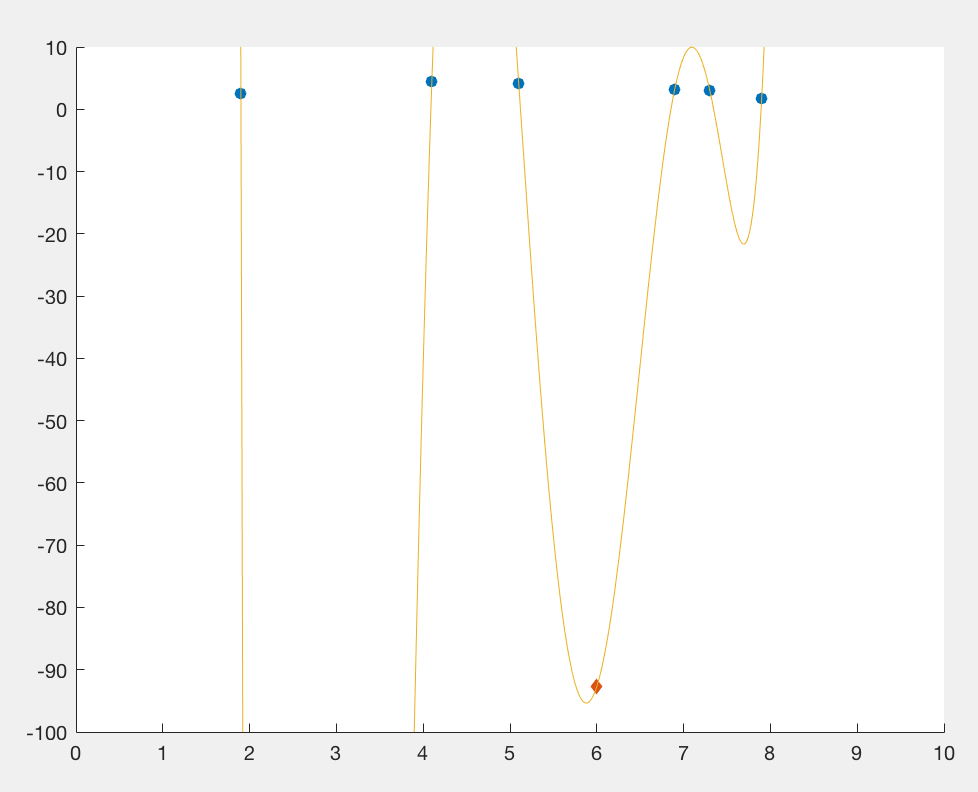
\includegraphics[width=12cm]{ass2clo2fig4} 
		\\

		\item (5 points) Between two models resulted from 15(a) and 15(b), which model that gives better prediction to p4? Why? Give your explanation.

		

		\par Gambar di bawah menampilkan prediksi dengan regresi linear dan regres non-linear menggunakan fungsi polinomial berderajat m = 7. Dari gambar, kita dapat melihat bahwa hasil prediksi regresi linear lebih dekat dengan \textit{data set} atau \textit{data latih}, dibandingkan dengan hasil prediksi regresi non-linear. Maka dari itu, menurut saya pada kasus di atas, prediksi menggunakan regresi linear lebih baik daripada regresi non-linear menggunakan fungsi polinomial berderajat m = 7.

		\par 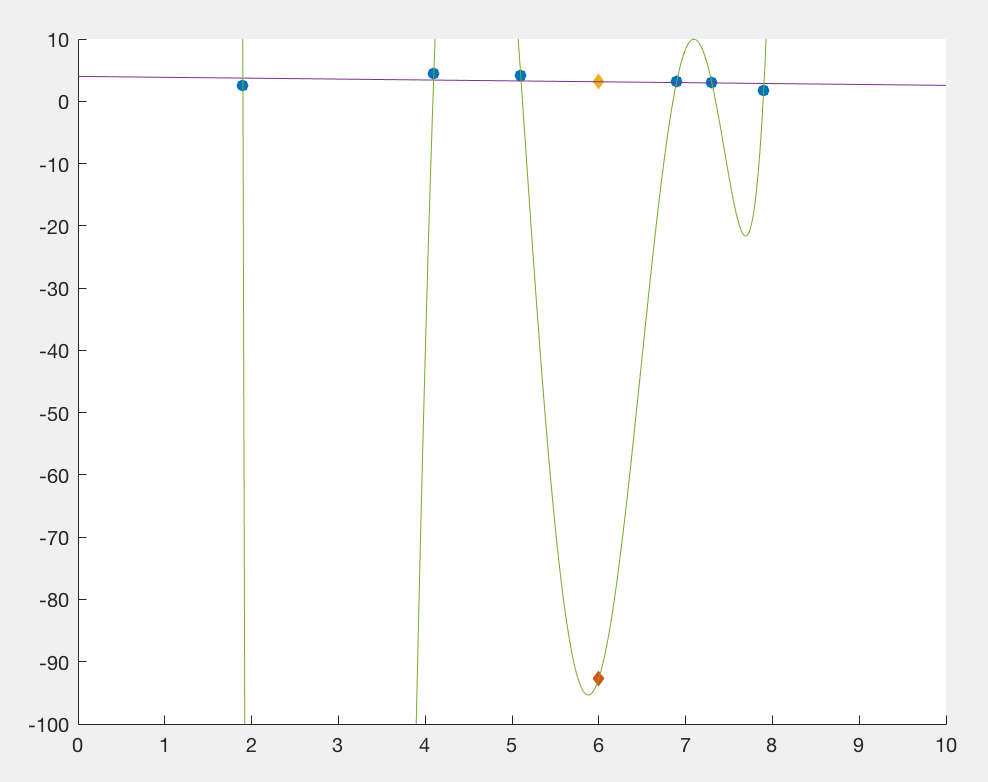
\includegraphics[width=12cm]{ass2clo2fig5} 
	\end{enumerate}

	\item Given data set 2 (xi, yi), where xi = (x1, x2), shown in Table 2.
	\begin{enumerate}
		\item (20 points) Build a multivariate linear regression model using data set 2 (except p4).
		\par Untuk membuat model linear, kita harus mencari nilai $\Omega$ terlebih dahulu. Nilai $\Omega$ dapat dicari menggunakan persamaan [2]

			\[\Omega = (\textup{X}^T\textup{X})^{-1}\textup{X}^Ty\]

		\par di mana $\Omega$ adalah 

			\[\Omega = (\omega_0, \omega_1)^T\]

		\par dan diketahui

			\[\textup{X} = \begin{pmatrix} 1& x_{11} & x_{12} & ... & x_{1d}\\ 1& x_{21} & x_{22} & ... & x_{2d} \\ ... & ... & ... & ... & ... \\ 1 & x_{N1} & x_{N2} & ... & x_{Nd} \end{pmatrix}\]

		\par Dengan memasukkan data latih ($x_1,x_2, \textup{dan} \ y$) yang ada di dataset, maka kita akan mendapatkan matriks

			\[\textup{X} = \begin{pmatrix} 1 & 3.2 & 5.8\\ 1 & 4.1 & 5.1\\ 1 & 5.1 & 4.0\\ 1 & 6.9 & 2.2\\ 1 & 7.3 & 1.7\\ 1 & 7.9 & 0.9 \end{pmatrix} , \textup{y} = \begin{pmatrix} 3.2\\ 4.5\\ 4.1\\ 3.2\\ 3\\ 1.8 \end{pmatrix}\]

		\par Menggunakan persamaan di atas,

			\begin{align*}
				\Omega & = \left ( \begin{pmatrix} 1 & 3.2 & 5.8\\ 1 & 4.1 & 5.1\\ 1 & 5.1 & 4.0\\ 1 & 6.9 & 2.2\\ 1 & 7.3 & 1.7\\ 1 & 7.9 & 0.9 \end{pmatrix} ^T \begin{pmatrix} 1 & 3.2 & 5.8\\ 1 & 4.1 & 5.1\\ 1 & 5.1 & 4.0\\ 1 & 6.9 & 2.2\\ 1 & 7.3 & 1.7\\ 1 & 7.9 & 0.9 \end{pmatrix} \right ) ^{-1} \begin{pmatrix} 1 & 3.2 & 5.8\\ 1 & 4.1 & 5.1\\ 1 & 5.1 & 4.0\\ 1 & 6.9 & 2.2\\ 1 & 7.3 & 1.7\\ 1 & 7.9 & 0.9 \end{pmatrix} ^T \begin{pmatrix} 3.2\\ 4.5\\ 4.1\\ 3.2\\ 3\\ 1.8 \end{pmatrix} \\
				& = \begin{pmatrix} -47.4041 \\ 5.5723 \\ 5.6842\end{pmatrix}
			\end{align*}

		\par dimana $\hat{\omega_0} = -47.4041,\hat{\omega_1} = 5.5723,\hat{\omega_2} = 5.6842$.

		\par 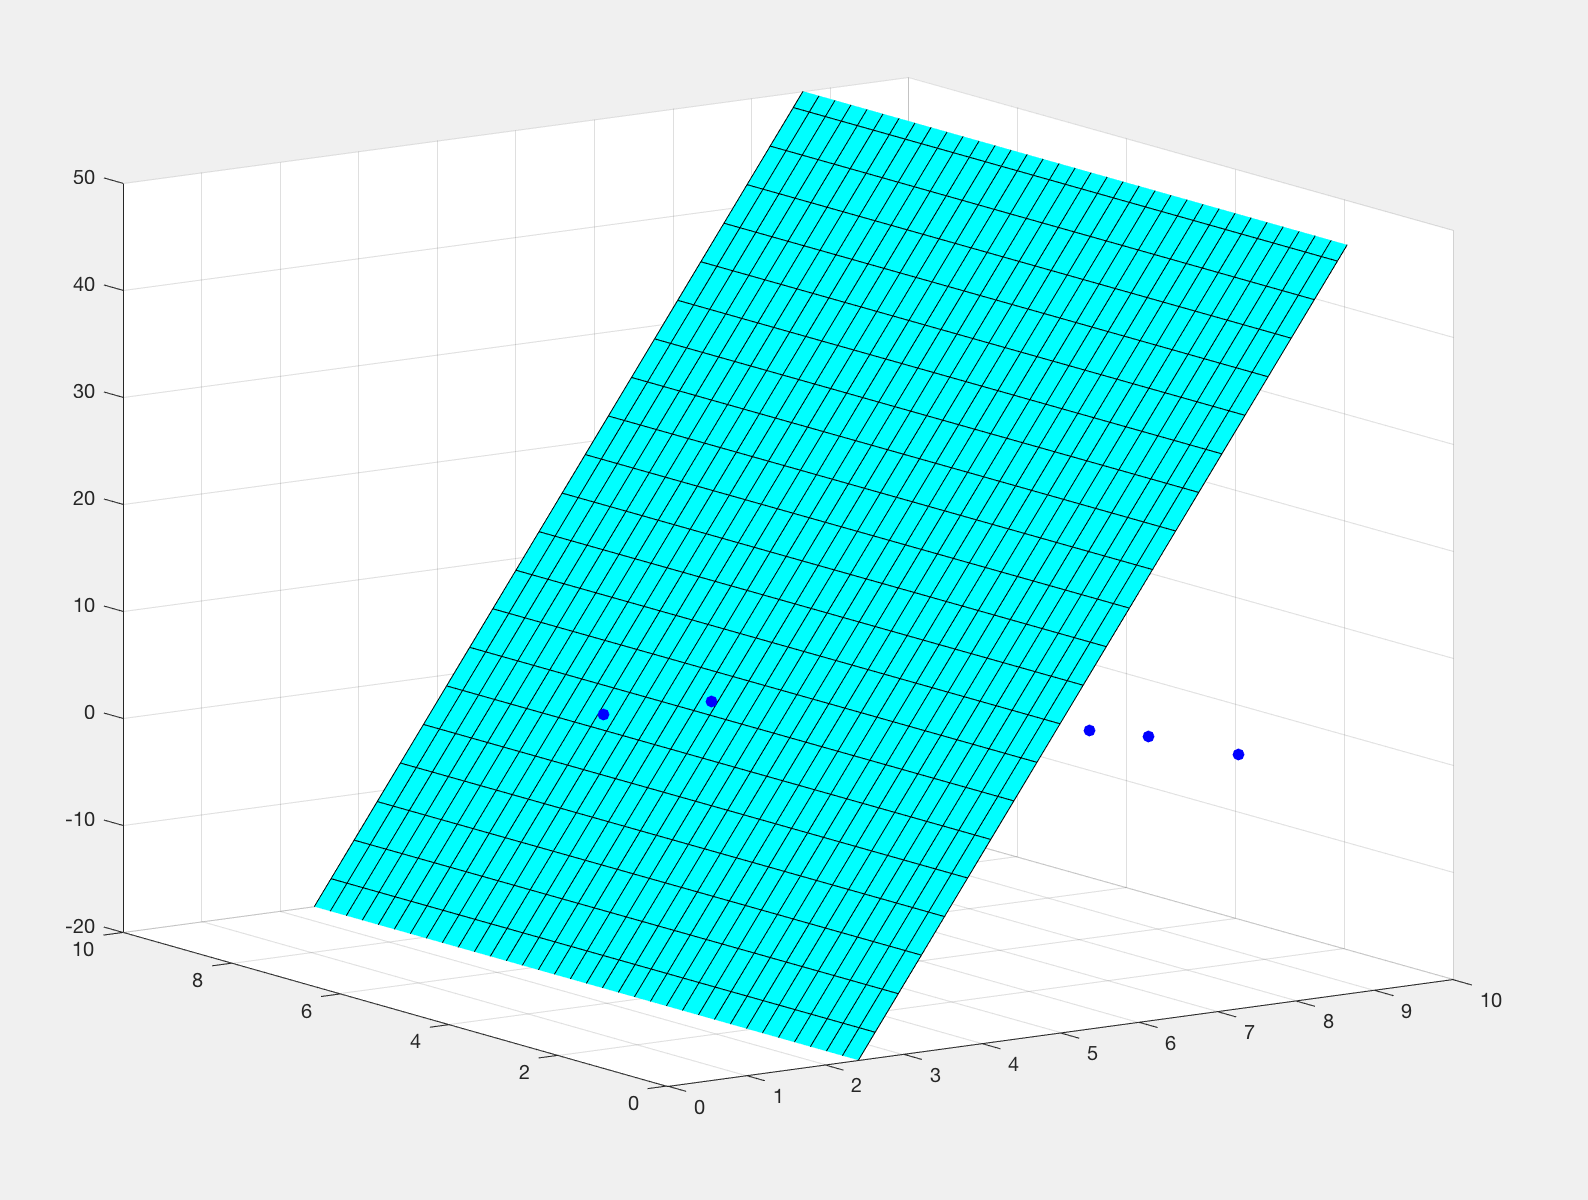
\includegraphics[width=10cm]{ass2clo2fig6} 

		\par 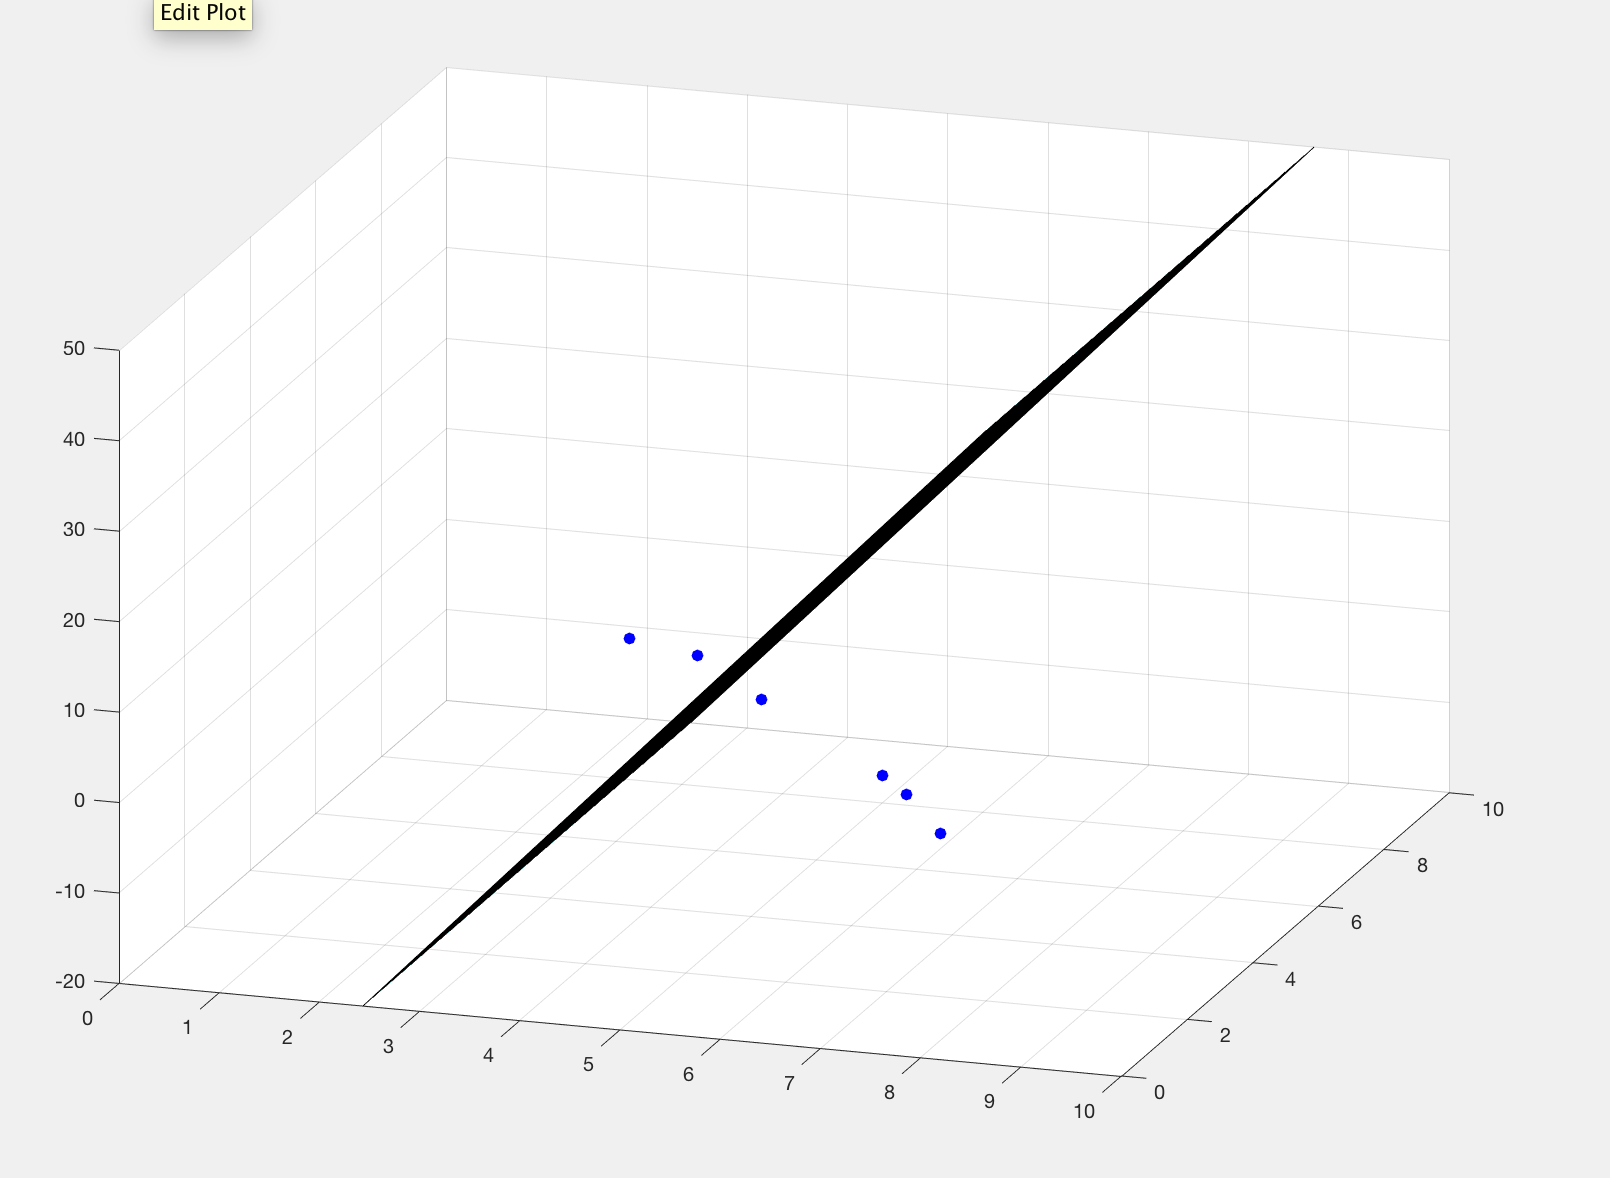
\includegraphics[width=10cm]{ass2clo2fig7} 

		\item (5 points) Predict the y value of p4 using model in 16(a).

		\par dengan menggunakan model di 16(a), nilai $y_4$ adalah $20.1353$.

		\par 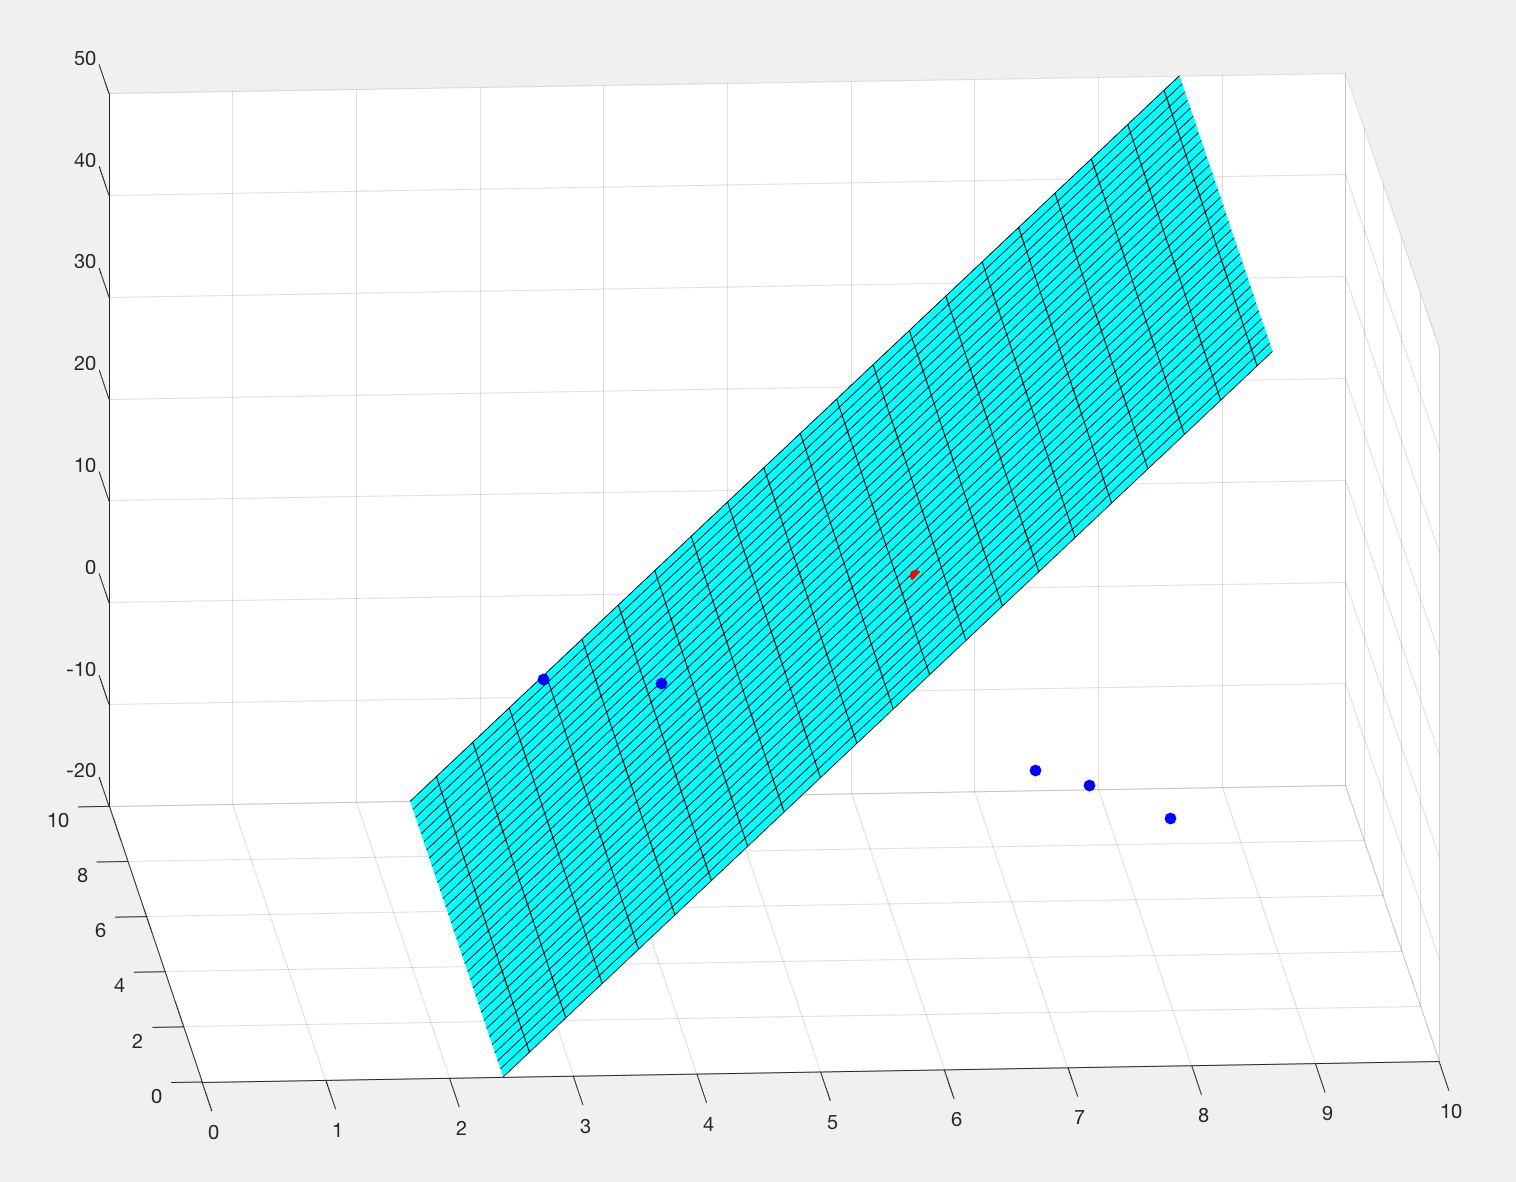
\includegraphics[width=10cm]{ass2clo2fig8} 		
		\par 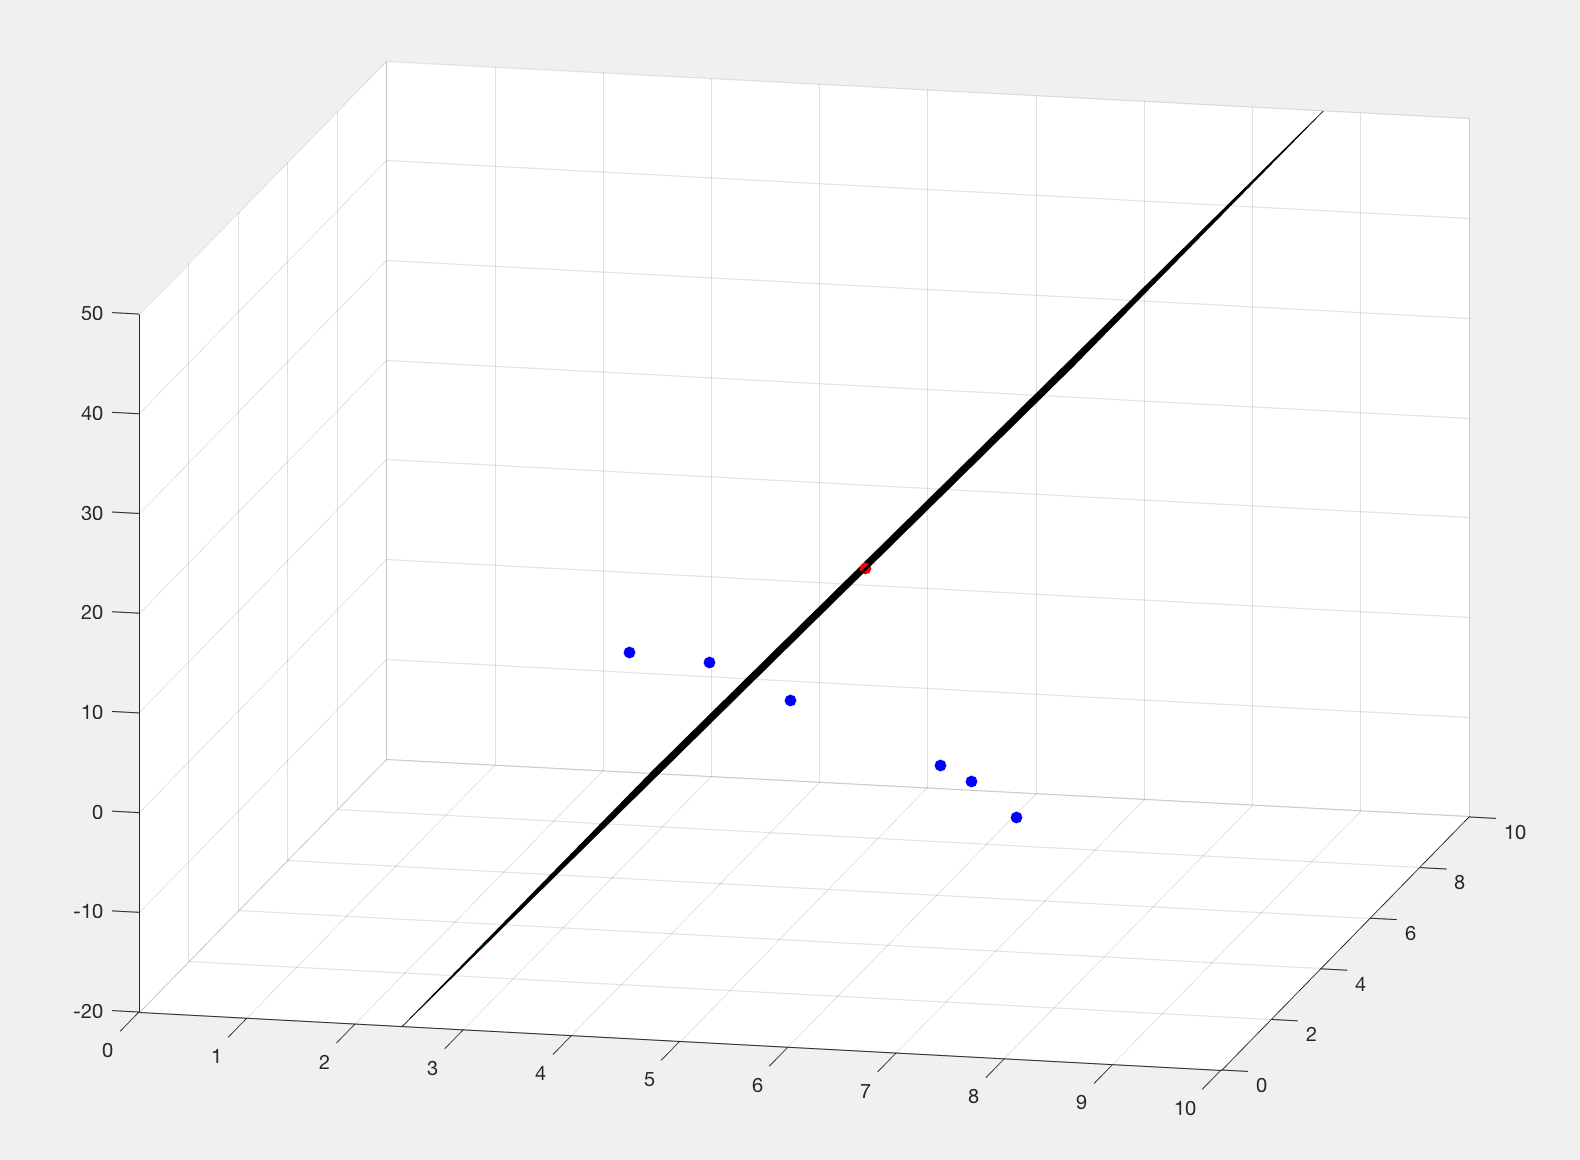
\includegraphics[width=10cm]{ass2clo2fig9} 


		\item (20 points) Build a multivariate non-linear regression model using data set 2 (except p4). (Hints: use some interaction terms as given in the slide of Regression page 17.)

		\par Dengan menggunakan rumus pada [5]

		\[y_i = f(\textup{x}_i) = \omega_0 + \omega_1x_{i1} + \omega_1x_{i2} + \omega_3x_{i1}x_{i2}\]

		\par dan menggunakan matriks masukan

		\[\textup{X} = \begin{pmatrix} 1 & x_{11} & x_{12} & x_{11}x_{12}\\ 1 & x_{21} & x_{22} & x_{21}x_{22} \\ 1 & x_{31} & x_{32} & x_{31}x_{32} \\ \vdots & \vdots & \vdots &\vdots \end{pmatrix} , \textup{y} = \begin{pmatrix} y_1\\ y_2\\ y_3\\ \vdots \end{pmatrix}\]

		\par kita dapat menggunakan persamaan pada 16(a) untuk mencari nilai $\Omega$

		\begin{align*}
		\scalemath{0.7}{
			\Omega & = \left ( \begin{pmatrix} 1&3.2&5.8&18.56 \\ 1&4.1&5.1&20.91 \\ 1&5.1&4&20.4 \\ 1&6.9&2.2&15.18 \\ 1&7.3&1.7&12.41 \\ 1&7.9&0.9&7.11 \\ \end{pmatrix} ^T \begin{pmatrix} 1&3.2&5.8&18.56 \\ 1&4.1&5.1&20.91 \\ 1&5.1&4&20.4 \\ 1&6.9&2.2&15.18 \\ 1&7.3&1.7&12.41 \\ 1&7.9&0.9&7.11 \\ \end{pmatrix} \right ) ^{-1} \begin{pmatrix} 1&3.2&5.8&18.56 \\ 1&4.1&5.1&20.91 \\ 1&5.1&4&20.4 \\ 1&6.9&2.2&15.18 \\ 1&7.3&1.7&12.41 \\ 1&7.9&0.9&7.11 \\ \end{pmatrix}^T \begin{pmatrix} 3.2\\ 4.5\\ 4.1\\ 3.2\\ 3\\ 1.8 \end{pmatrix} \\
			& = \begin{pmatrix} -23.3572 \\ 2.7489 \\ 2.6568 \\ 0.1350\end{pmatrix}}
		\end{align*}

		\par dimana $\hat{\omega_0} = -23.3572,\hat{\omega_1} = 2.7489,\hat{\omega_2} = 2.6568,\hat{\omega_3} = 0.1350$.

		\par 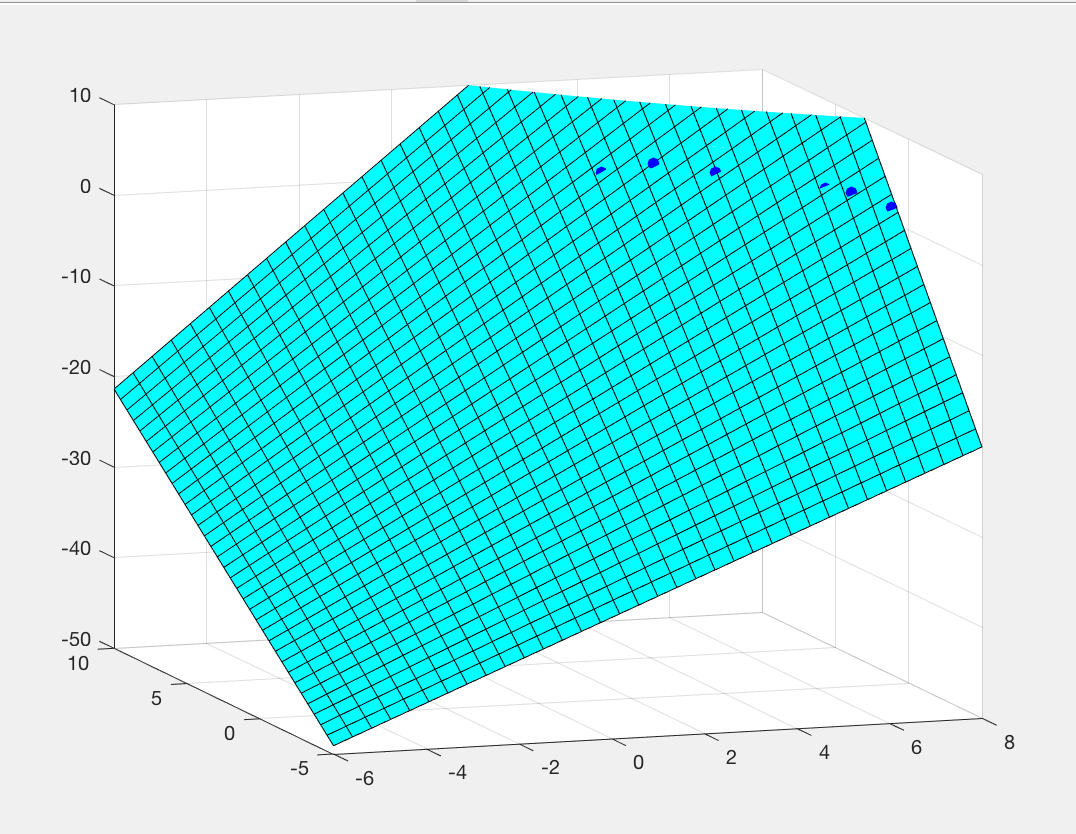
\includegraphics[width=10cm]{ass2clo2fig10} 
		\par 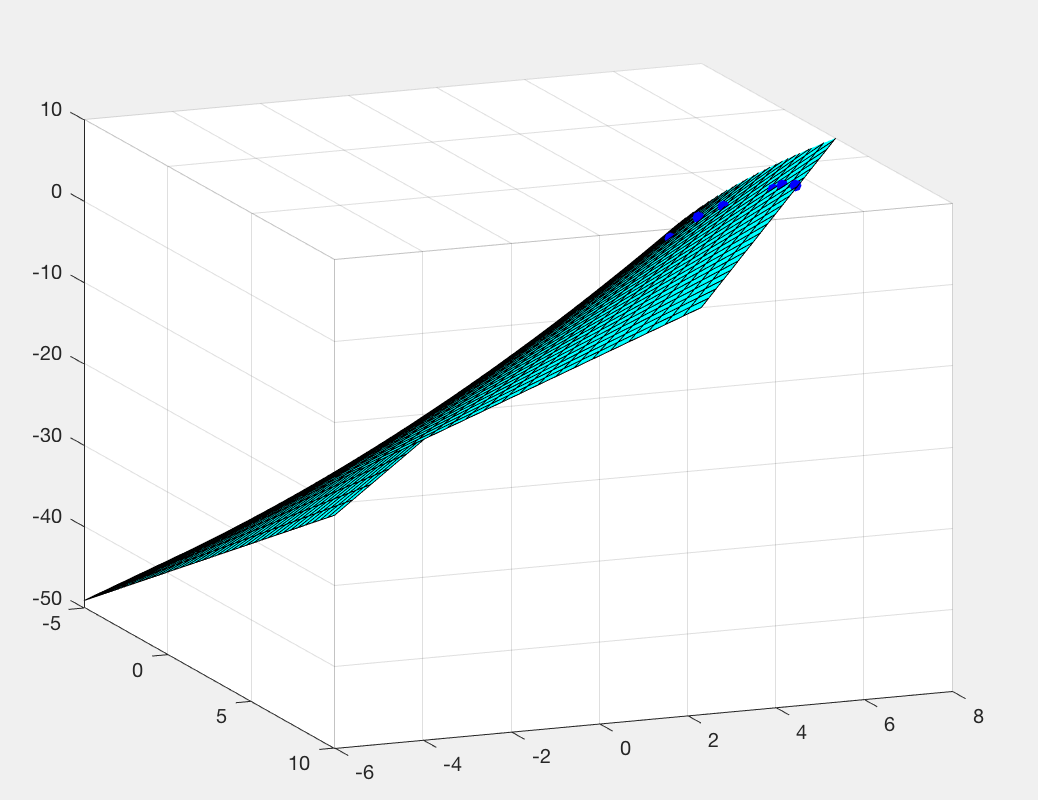
\includegraphics[width=10cm]{ass2clo2fig11} 

		\item (5 points) Predict the y value of p4 using multivariate non-linear regression model in 16(c).

		\par Dengan menggunakan model di 16(c), nilai $y_4$ adalah $3.88328$;

		\par 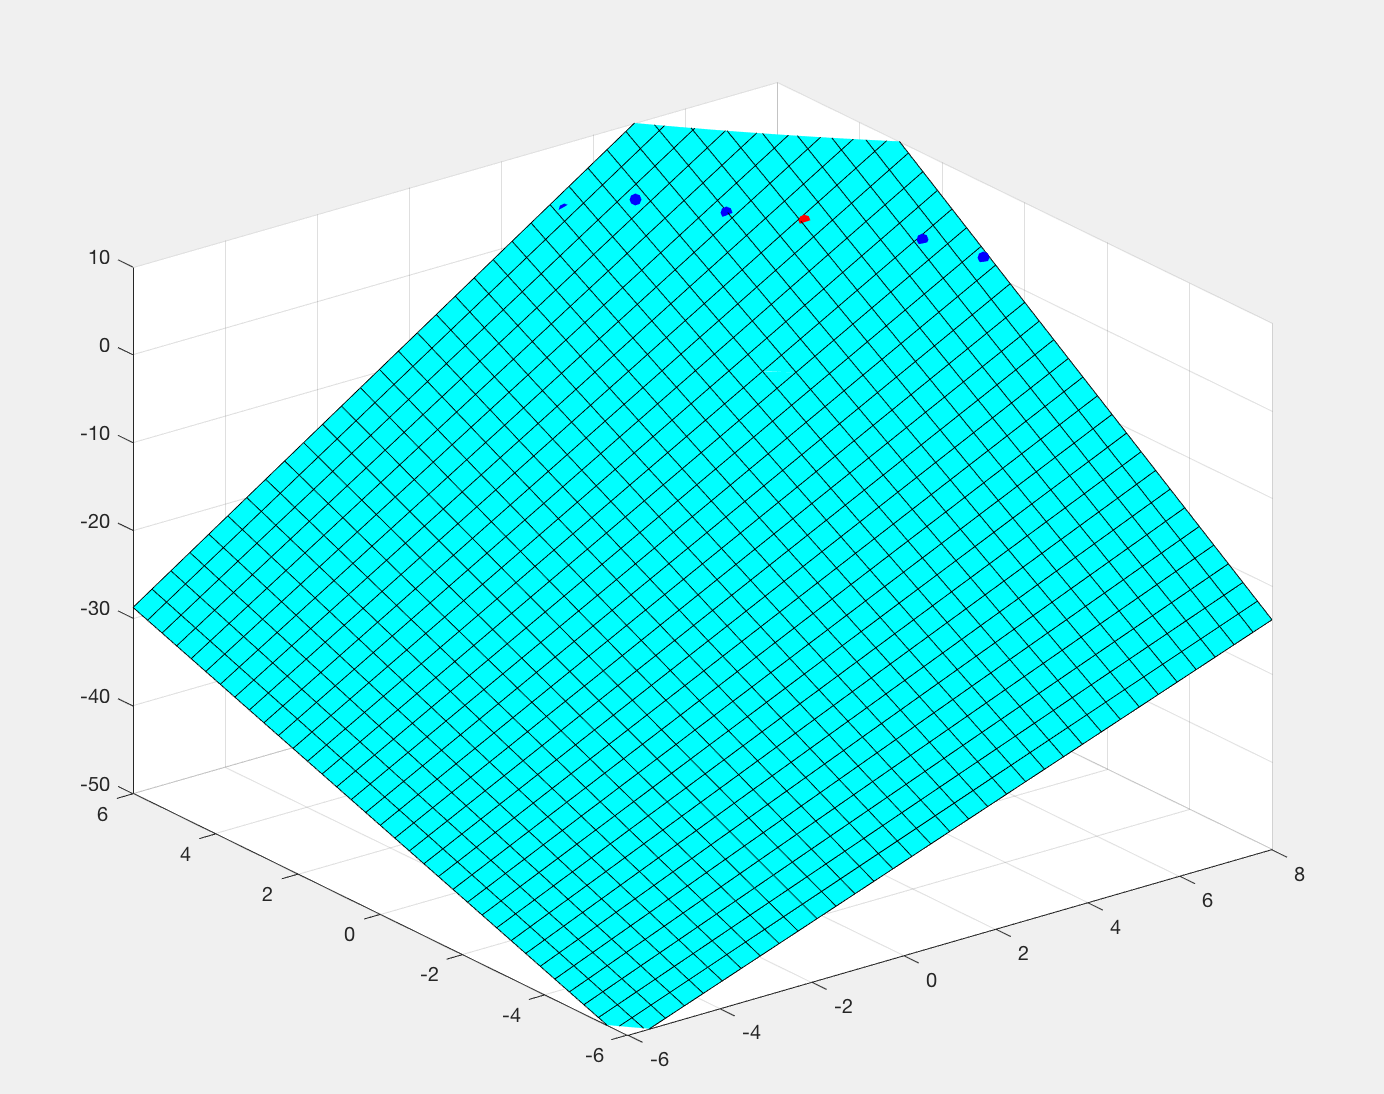
\includegraphics[width=10cm]{ass2clo2fig12} 
		\par 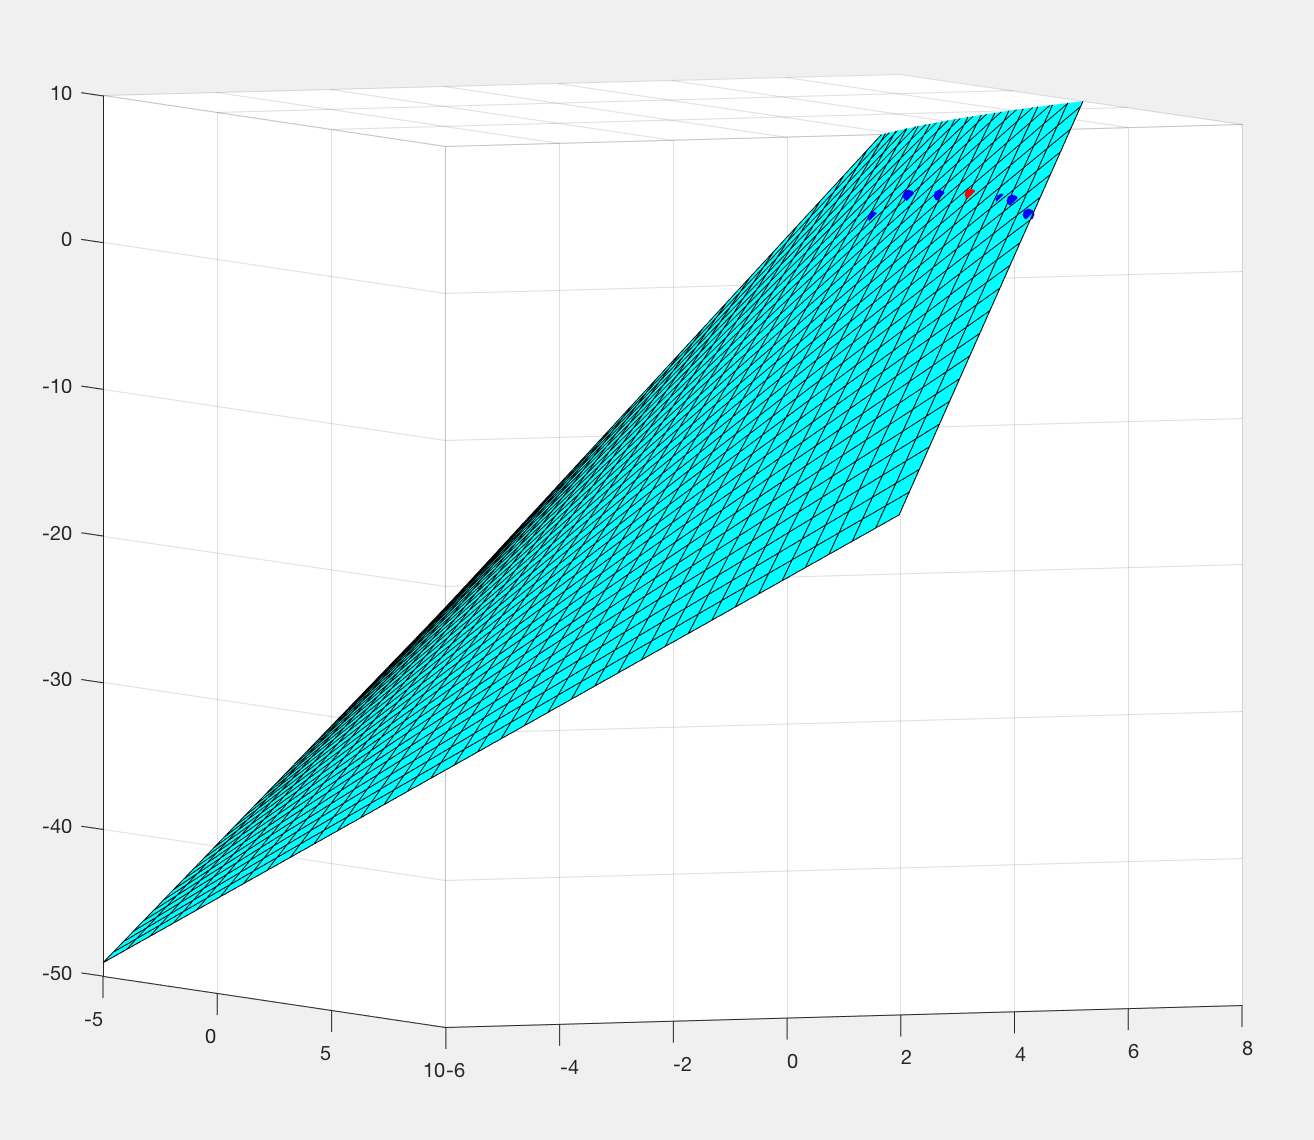
\includegraphics[width=10cm]{ass2clo2fig13} 

		\item (5 points) Between two models resulted from 16(a) and 16(c), which model that gives better prediction to p4? Why? Give your explanation.

		\par Dari grafik, dapat dilihat bahwa model 16(c) mempunya nilai prediksi yang mendekati nilai-nilai dataset atau datatraining. Menurut saya, model 16(c) lebih baik daripada 16(a)

		\par 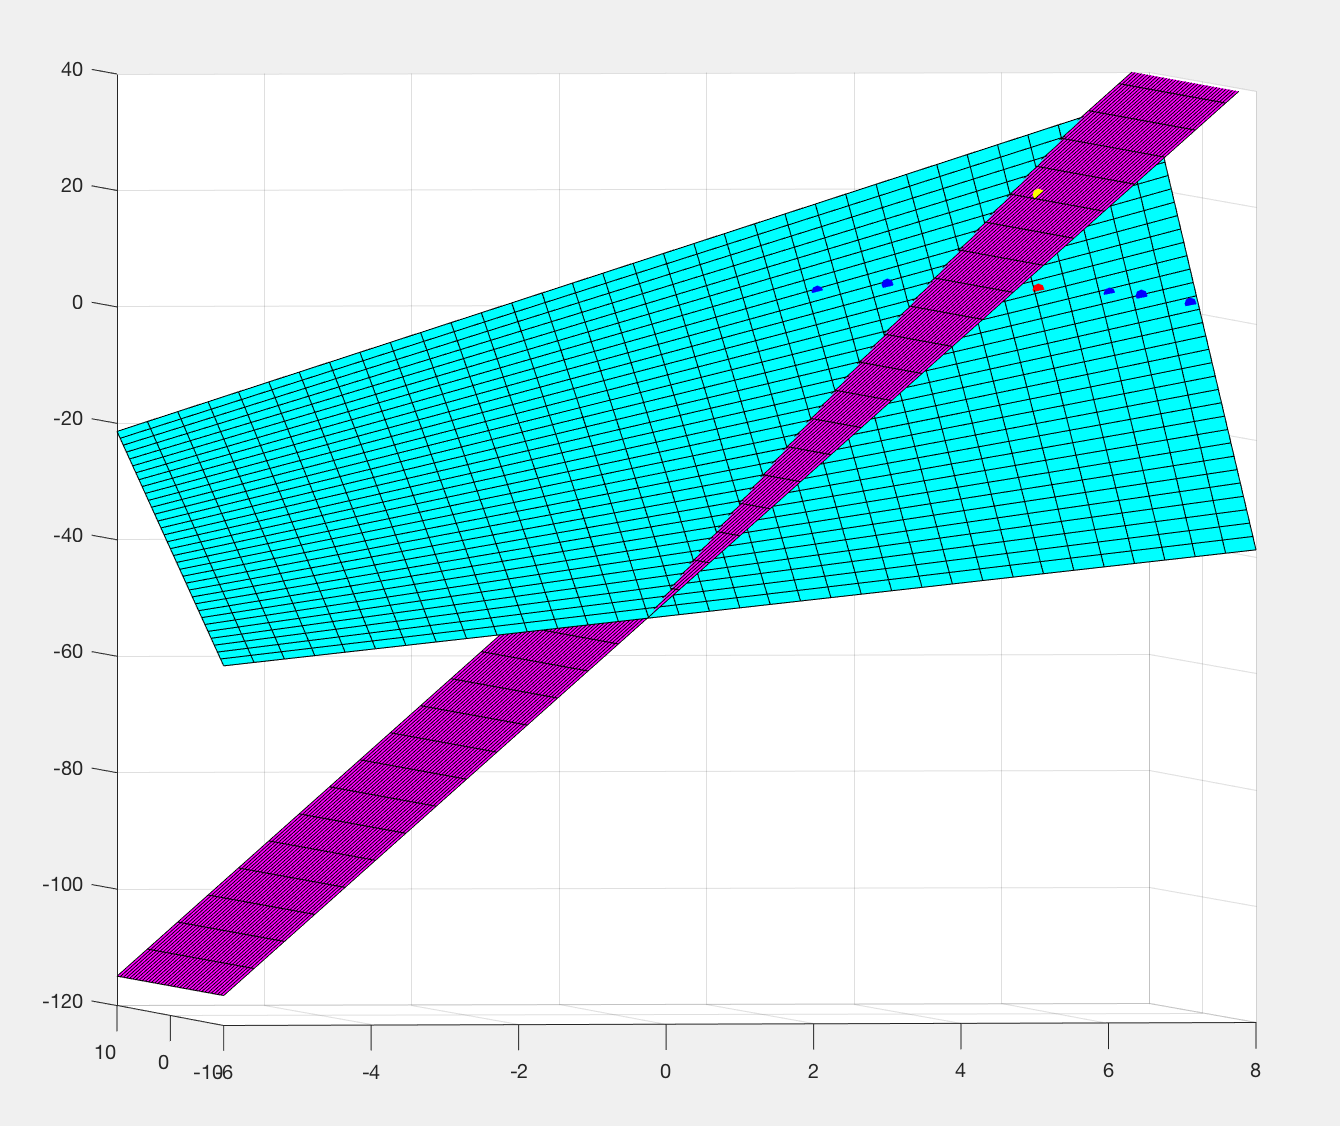
\includegraphics[width=10cm]{ass2clo2fig14} 
		\par 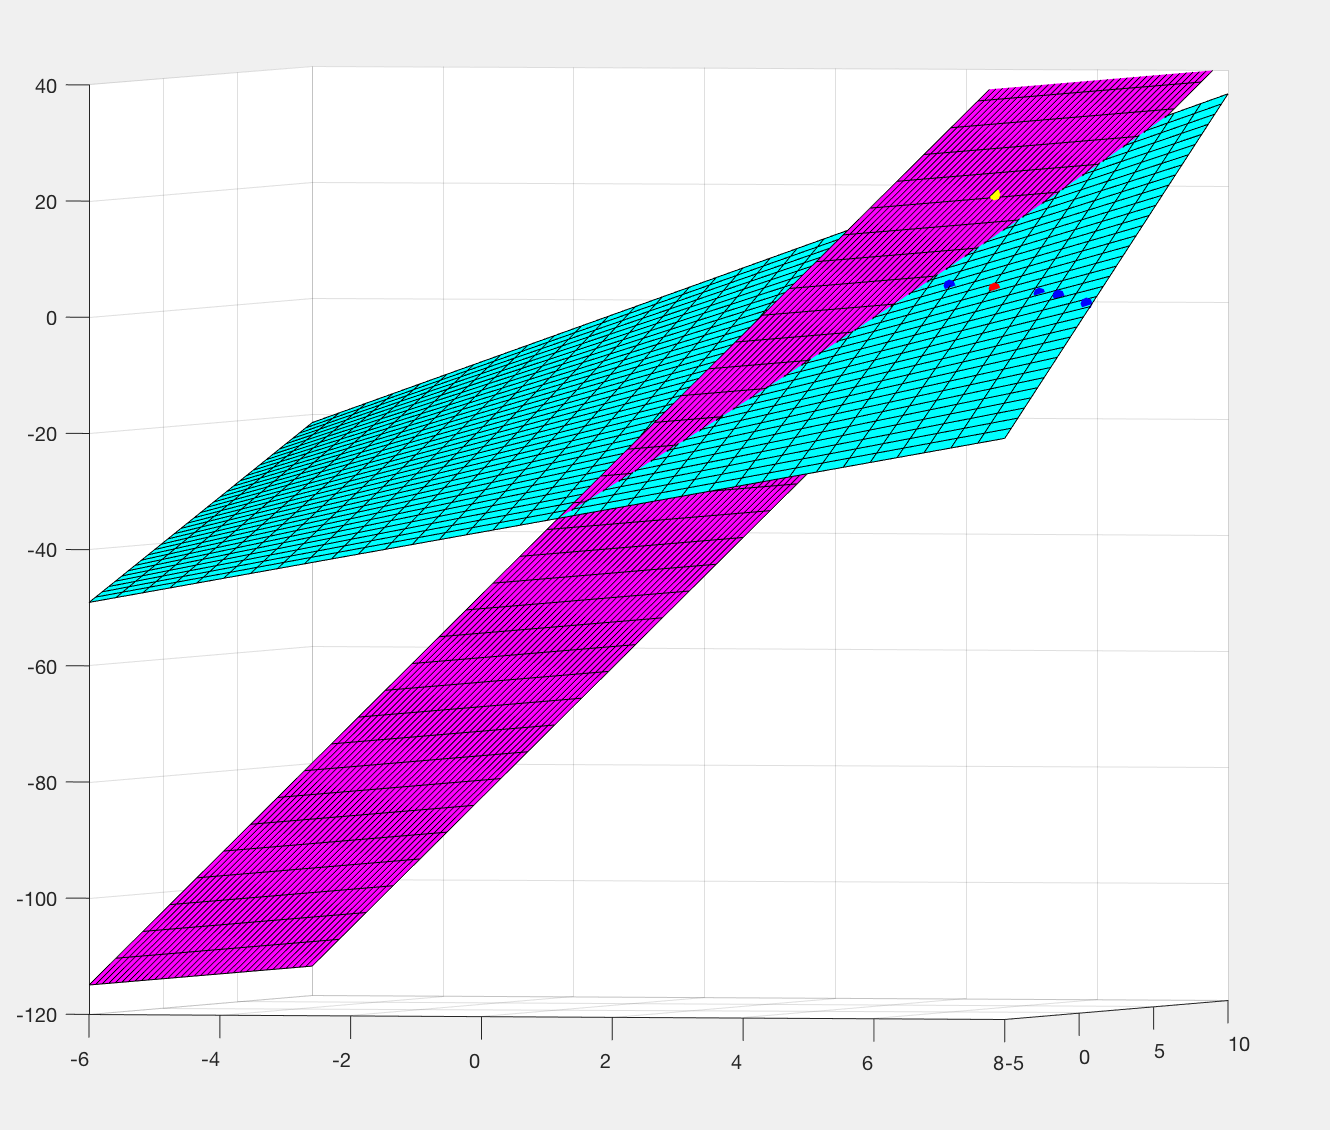
\includegraphics[width=10cm]{ass2clo2fig15} 
	\end{enumerate}


\end{enumerate}

\par \textbf{Referensi}
\par [1] https://id.wikipedia.org/wiki/Regresi_Linier
\par [2] Introduction to Data Mining - Panning Tan, M. Steinbach
\par [3] https://en.wikipedia.org/wiki/Nonlinear_regression
\par [4] Regression book
\par [5] Regression slide
\par [6] http://www.nickgillian.com/wiki/pmwiki.php/GRT/MLP
\par [7] Machine Learning - Tom Mitchell
\par [8] https://medium.com/towards-data-science/activation-functions-and-its-types-which-is-better-a9a5310cc8f
\par [9] Slide ANN-MLP Machine Learning

\end{document}

